\newpage
\section{Results}
After applying the methods described in the previous section \ref{github_method}, three open source implementations were selected for evaluation: TorToise\cite{betker_tortoise_2022}, VALL-E (X)\cite{songting_vall-e_2023} and Real-Time Voice Cloning\cite{jemine_corentinjreal-time-voice-cloning_2023}. All three offer pretrained models and support English synthesis. While TorToise and VALL-E (X) are actively maintained, Real-Time Voice Cloning, an older tool, was chosen for comparative analysis with the more recent implementations. In this section, we delve into each open-source implementation, starting with a comprehensive description of their respective model architectures. Following this, a thorough assessment of usability and ease of use is conducted. Conclusively, the models are evaluated as described in \ref{eval_method}. All synthesis tasks were performed on an NVIDIA GeForce MX350 with 2GB VRAM.

In table \ref{tab:comparison_table} the results and characteristics of the three open-source implementations are summarized.

\begin{table}[h!]
    \centering
    \begin{tabular}{|lccc|}
    \hline
         & TorToise & VALL-E (X) & Real-Time Voice Cloning \\
    \hline
         Intermediate representation&mel-spectrograms&acoustic tokens&mel-spectrograms\\
         Training data (only English)&49'896 h&704 h&2960 h \\
         Long text synthesis&\ding{51}&\ding{51}&\ding{51} \\
         Quality selection&\ding{51}&\ding{55}&\ding{55} \\
         Prompt engineering for emotions&\ding{51}&\ding{55}&\ding{55} \\
         Cross-lingual synthesis&\ding{55}&\ding{51}&\ding{55} \\
         Synthesis time (average)&110 minutes&170 seconds&10 seconds\\
         Naturalness of output&high&medium&low\\
         Similarity to target voice&medium&medium&low\\
         Expressiveness of output&low-medium&medium&low\\
    \hline
    \end{tabular}
    \caption{Comparison of the three open-source implementations TorToise, VALL-E (X) and Real-Time Voice Cloning}
    \label{tab:comparison_table}
\end{table}

\subsection{TorToise}
The author of TorToise\cite{betker2023better} states that TorToise is a \gls{tts} System that combines an auto-regressive decoder with a \gls{ddpm}, both often used in image generation models.
The auto-regressive decoder utilizes a GPT-2 architecture for generating speech tokens based on the target text and on audio clips of the target speaker. The \gls{ddpm} is used as the acoustic model to generate mel-spectrograms and Univnet as the vocoder.

During inference the auto-regressive decoder generates a large number of speech tokens. The highest quality speech token is then selected using Contrastive Language-Voice Pretrained Transformer (CLVP), a model similar to CLIP from DALL-E. The selected speech tokens are then fed into the \gls{ddpm} and finally Univnet generates the audio waveforms.

TorToise is trained on a dataset comprising LibriTTS, HiFiTTS, which combined give 896 hours of transcribed speech, and an extended dataset of 49'000 hours of cleaned audio from audiobooks and podcasts, transcribed with a wav2vec2-large model.

The author of TorToise further highlights the extreme slowness of the tool compared to other \gls{tts} systems, attributed to the use of both an auto-regressive decoder and a diffusion decoder.
Furthermore, driven by ethical concerns about potential misuse of the voice-cloning text-to-speech system, he created Tortoise-detect, a classifier model to detect if a speech was generated by TorToise. For the same reason he refrains from releasing training configuration details of TorToise\cite{betker_tortoise_2022}.

\subsubsection{Ease of use}

\textbf{Installation}: To utilize the latest version of TorToise, users can either install it locally or access an  official live demo hosted on Hugging Face Spaces\cite{betker_tortoise_hugging_face}. The demo hosted on Hugging Face Spaces does not offer certain features, such as cloning a custom voice and selecting presets, which affect the quality of the generated speech. An alternative demo of TorToise hosted on Replicate\cite{mullis_afiaka87tortoise-tts_nodate} include these features but does not have the latest TorToise version. Therefore the tool was installed locally in a conda environment following the repository README\cite{betker_tortoise_2022}.

\textbf{Main features}: The key features of TorToise are:
\begin{itemize}
    \item Generation of a sentence or a large text file with one or more voices separately.
    \item Combination of multiple voices when generating a speech.
    \item Use of four different presets (ultra\textunderscore fast, fast, standard, high\textunderscore quality). The presets differ in the number of speech tokens generated by the auto-regressive decoder, and in the number of iterations of the \gls{ddpm}. These factors affect the quality of the generated speech and the synthesis time.
    \item Selection of the number of output candidates to generate.
    \item Prompt engineering to generate speech with emotions.
\end{itemize}

\textbf{User interface}: The locally installed tool does not offer a \gls{gui} and can only be used via terminal instructions.

\textbf{Accessibility of documentation}: Documentation on how to use the model is available on the repository\cite{betker_tortoise_2022}. The README provides well-documented installation instructions. Although the author of TorToise specifies the need for an NVIDIA GPU, our tests with CPUs produced comparable results, albeit with longer synthesis times. The documentation describes how to add custom voices. The terminal commands for the generation of speech are listed in the documentation. However, additional command arguments, such as presets selection and the number of output candidates, are not extensively detailed and require the consulting of the source code for more information. In the documentation, a brief section is dedicated to utilizing prompt engineering for emotions. However, a detailed list of all supported emotions is absent, apart from a few examples provided by the author.

\subsubsection{Generated speech}
%General description of all the samples, were there really bad ones, really good ones.
%Were there differences in quality when worsening the input quality?
%Which settings were used / which settings produced best outcome?
%What are the generated times?
All generated speeches were produced using the high\textunderscore quality preset. In each synthesis three output candidates were generated and the optimal result was manually selected for evaluation.

When using high-quality monotone audio as target voice, the generated speeches exhibit a natural sounding voice with both male and female voices. Although the voices of the generated speeches bear a resemblance to the target voices, they are distinguishable upon attentive listening. Notably, the monotonous tone of the original voice is altered, adopting a book reading style with increased emphasis on certain words. This book reading style is less pronounced with the female voice. Some of the generated speeches manifest a British accent, a feature not present in the reference voice.

\todo[inline]{DONE. IS OK? more human sounding but not necessarily more target sounding}

Speeches generated using telephone-quality audio as reference similarly retain the book reading style. Moreover, the audio sounds more distorted than the reference audio, significantly diminishing the voice similarity to the target voice.

Attempts to generate speech with an angry emotion yielded mixed results. Firstly, when using an angry-voiced audio as reference, the original voice was not preserved very well in the output. The voice did not sound similar to that of the target and the emotion of anger was not as evident as in the original audio. Alternatively, employing prompt engineering with a neutral-voiced reference, and appending "[I am so angry,]" to the text, produced a more faithful reproduction of the original voice. However, there was not the intended emotion of anger.

Using a longer audio as reference didn't affect the quality and naturalness of the generated speech.

The synthesis of one sentence with the preset high\textunderscore quality takes on average about 110 minutes, going from 66 minutes for the shortest sentence (pangram2) to 160 minutes for the longest sentence (pangram4).

% requirements for audio clips of your voice https://github.com/neonbjb/tortoise-tts/blob/main/voice_customization_guide.md




\subsection{VALL-E (X)}
VALL-E\cite{wang2301neural} is a recent TTS framework introduced by Microsoft, that differs from previous TTS frameworks in its distinctive approach to synthesizing speech. Instead of treating TTS as a continuous signal regression, where mel-spectograms are generated and used as an intermediate representation, VALL-E treats TTS as a conditional language modeling task, generating acoustic tokens.

\begin{figure}[h!]
    \centering
    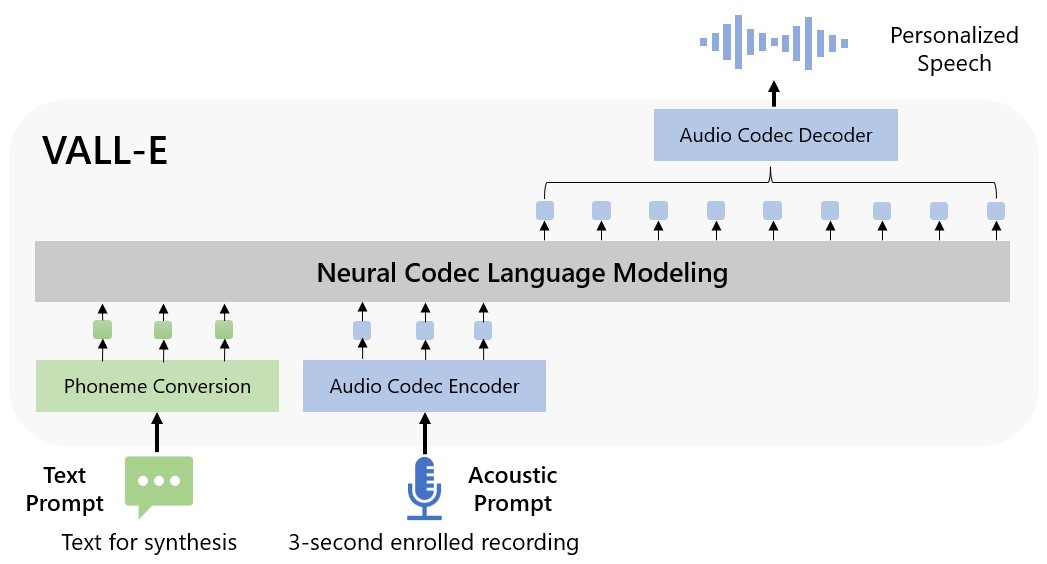
\includegraphics[width=1\linewidth]{assets/VALLE_Overview.jpg}
    \caption{Inference process of VALL-E\cite{wang2301neural}}
    \label{fig:valle_overview}
\end{figure}

Figure \ref{fig:valle_overview} shows the inference process of VALL-E: the text to synthesize and a few seconds of speech of the target speaker are taken as input. The text input and the acoustic input are respectively converted into phonemes and acoustic tokens. Based on these phonemes and acoustic tokens, VALL-E generates additional acoustic tokens, which are fed into the audio codec decoder to synthesize personalized speech. The Neural Codec Language Model (the grey rectangle) comprises an auto-regressive Transformer and a non-auto-regressive Transformer. EnCodec\cite{defossez2022high} is used as the Audio Codec Encoder/Decoder (blue rectangles). 

Although there is no official public implementation of VALL-E, several unofficial open-source implementations are available on GitHub\cite{valle, niu_vall-e_2023, songting_vall-e_2023}. To test the VALL-E framework this GitHub repository\cite{songting_vall-e_2023} was selected, primarily because it offers a pretrained model. It is essential to note that this particular repository implements VALL-E X\cite{zhang2023speak}, an extension of VALL-E that enables cross-lingual speech synthesis, i.e. speech synthesis in a language different from the source speaker's language. The inference process remains similar to VALL-E, the only difference being that the transcription of the input speech and the target language ID are additionally given as input. The author of the repository replaced the EnCodec decoder with a Vocos decoder\cite{siuzdak2023vocos}, stating it improved the audio quality. 

The pretrained model of the unofficial implementation was trained on 704 hours of English speech from LibriTTS and self-gathered audios, on 598 hours of Chinese speech from  AISHELL-1, AISHELL3, Aidatatang and self-gathered audios, and on 437 hours of Japanese speech from Japanese Common Voice and self-gathered audios\cite{noauthor_demo_nodate}.

\subsubsection{Ease of use}
\textbf{Installation}: The author of the repository provide a demo hosted on Hugging Face Spaces\cite{vallex_hugging_face}. Alternatively, users can follow the instructions in the README of the repository for local installation\cite{songting_vall-e_2023}. To benchmark synthesis time against the other open-source implementations, it was decided to install VALL-E X locally in a conda environment.

\textbf{Main features}:
The key features of VALLE X are:
\begin{itemize}
    \item Sentence or long text generation with a single voice.
    \item Cross-lingual speech synthesis.
    \item Accent selection of the generated speech.
    \item Downloading the encoded prompt, allowing the skipping of the encoding process in subsequent inferences with the same acoustic prompt.
\end{itemize}

\textbf{User interface}:
This implementation can be used directly in Python or through a \gls{gui}. The latter option streamlines the synthesis process for users unfamiliar with command-line terminals.

\textbf{Accessibility of documentation}: Comprehensive documentation for the tool is available in the repository\cite{songting_vall-e_2023}. It covers the use of the tool in Python code and details its features. In the documentation, the author refers to this repository\cite{valle} for the training code to train an own model.

\subsubsection{Generated speech}
All generated speeches were produced using the no-accent setting for the output.

Speeches generated with VALL-E X yielded mixed results. Notably, VALL-E X introduced a breathing sound at the start of some outputs, enhancing the realism of the speech, even if the reference audio lacked this characteristic. However, VALL-E X struggled in generating pangram3 and pangram4, exhibiting instances of slurred articulation and mispronouncing words, leading to an unnatural delivery. The audio quality, while generally good, did not match the crispness observed with TorToise, and some outputs exhibited a hoarse quality in the male voice. The female voice displayed a higher level of similarity to its reference voice than the male voice, but noticeable differences are apparent to someone familiar with the original speaker.

When using telephone-quality audio as a reference, the output speech took on a more robotic quality, but still performed better than TorToise.

Generating speech with an angry tone, using an angry-voiced reference audio resulted in a more dissimilar output voice compared to TorToise. However, VALL-E X performed better in reproducing the emotion of anger.

Using a longer audio as a reference, in some cases, negatively impacted the naturalness of the generated speech.

The synthesis time of one sentence averages about 170 seconds, ranging from 90 seconds for the shortest sentence (pangram2) to 220 seconds for the longest sentence (pangram4). In contrast to TorToise, in VALL-E X at times, the initial synthesis may fail to produce an optimal output, requiring multiple attempts (typically around three) to achieve a satisfactory result.

\begin{figure}
\centering
\begin{subfigure}{0.49\textwidth}
\centering
\includegraphics[width = \textwidth]{assets/visualization_original3.png}
\caption{Original voice of pangram3}
\label{fig:visualization_original3}
\end{subfigure}
\begin{subfigure}{0.49\textwidth}
\centering
\includegraphics[width = \textwidth]{assets/visualization_valle3.png}
\caption{Generated output from pangram2}
\label{fig:visualization_valle3}
\end{subfigure}
\caption{Wavegram and Mel-spectrogram of pangram3}
\label{fig:visualization_valle}
\end{figure}

\subsection{Real-Time Voice Cloning}
Real-Time Voice Cloning is the result of a Master Thesis\cite{jemine2019master} from 2019, where the author implements the framework described in this work\cite{jia2018transfer} from 2018 by Google.
As illustrated in figure \ref{fig:rtvc_framework} the framework consists of:

\begin{itemize}
    \item A speaker encoder, based on GE2E (Generalized End-To-End Loss)\cite{wan2018generalized}, that takes as input a few seconds of speech of the target speaker and generates an embedding vector containing the speaker's characteristics.
    \item An acoustic model, in the work referred to as a synthesizer, based on a modified version of Tacotron 2, where the embedding vector is concatenated to the acoustic model in the attention layer. 
    \item A vocoder based on WaveRNN, differing from the original work by Google\cite{jia2018transfer} which used WaveNet. 
\end{itemize}

\begin{figure}[h!]
    \centering
    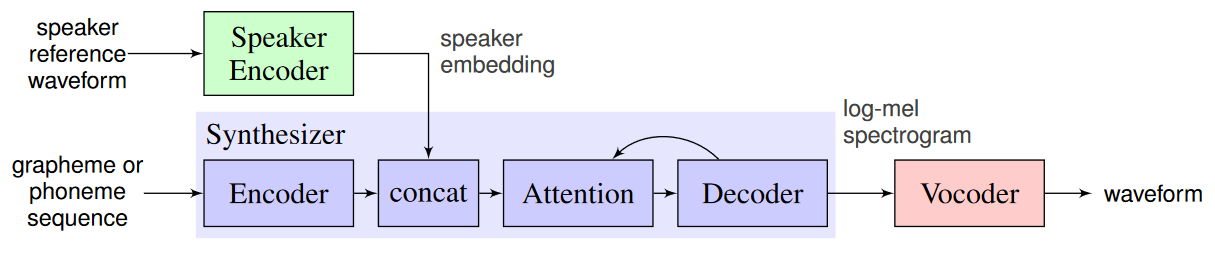
\includegraphics[width=1\linewidth]{assets/realtime voice cloning inference.png}
    \caption{framework components\cite{jia2018transfer}}
    \label{fig:rtvc_framework}
\end{figure}

The three components were trained independently. The speaker encoder was trained on the three datasets LibriSpeech-Other, VoxCeleb1 and VoxCeleb2, which combined give over 2'500 hours of audio. The acoustic model and the vocoder were trained on 460 hours of audio from the LibriSpeech-Clean Dataset.
%TODO reference all datasets.

\subsubsection{Ease of use:}

\textbf{Installation}: Setting up Real-Time Voice Cloning locally in a conda environment proved challenging due to missing dependencies and incompatible versions listed in the requirements.txt file. The installation process involved manual installation of missing modules and adjustment of library versions.

\textbf{Main features:}
The key featurs of Real-Time Voice Cloning are:

\begin{itemize}
    \item Sentence or long text generation with a single voice.
    \item Visualization of mel-spectograms and embeddings for both the reference and generated audio.
    \item Visualization of embeddings in a 2D-space, where embeddings from the same speaker are grouped into clusters.
\end{itemize}

\textbf{User interface}: While the tool includes a \gls{gui} toolbox for generating personalized speech, compatibility issues prevent the toolbox from functioning on Windows 11 due to the repository's lack of maintenance. The tool can be used via terminal commands, but without access to the visualization features mentioned above.

\textbf{Accessibility of documentation}: The README of the repository\cite{jemine_corentinjreal-time-voice-cloning_2023} contains a concise video explaining the toolbox. For detailed information on training configurations and instructions to train a personalized model, users can refer to the repository's Wiki.

\subsubsection{Generated speech}
All the speeches generated with Real-Time Voice Cloning yielded poor results. All outputs present a robotic, hoarsed voice with a quick pace and slurred articulation. The original voice is very slightly resembled in the generated speech, but because of the robotic rhythm, the speeches don't show any naturalness.
Using an angry-voiced reference does not affect the emotion of the generated speeches, which always have a monotone emotion.

To synthesise one sentence Real-Time Voice Cloning takes about 10 seconds.

The outputs of the speech synthesis process using Real-Time Voice Cloning consistently yielded unsatisfactory results. The generated speeches consistently display a robotic, hoarse voice characterized by a rapid pace and slurred articulation. While there exists a subtle resemblance to the original voice, the outputs lack the natural cadence inherent in human speech, primarily attributed to the persistent robotic rhythm.

When an audio with an angry voice was utilized as a reference, the emotion in the generated speeches remained consistently monotone, indicating a limitation in conveying emotions.

The synthesis of a single sentence through Real-Time Voice Cloning requires approximately 10 seconds. Generating multiple candidates for a sentence by manually running multiple inferences did not improve the result.

\begin{figure}
\centering
\begin{subfigure}{0.49\textwidth}
\centering
\includegraphics[width = \textwidth]{assets/visualization_original1.png}
\caption{Original voice of pangram1}
\label{fig:visualization_original1}
\end{subfigure}
\begin{subfigure}{0.49\textwidth}
\centering
\includegraphics[width = \textwidth]{assets/visualization_rtvc1.png}
\caption{Generated output from pangram3}
\label{fig:visualization_rtvc1}
\end{subfigure}
\caption{Wavegram and Mel-spectrogram of pangram1}
\label{fig:visualization_rtvc}
\end{figure}
